\section{Background}\label{sec:background}
\begin{figure}
    \centering
    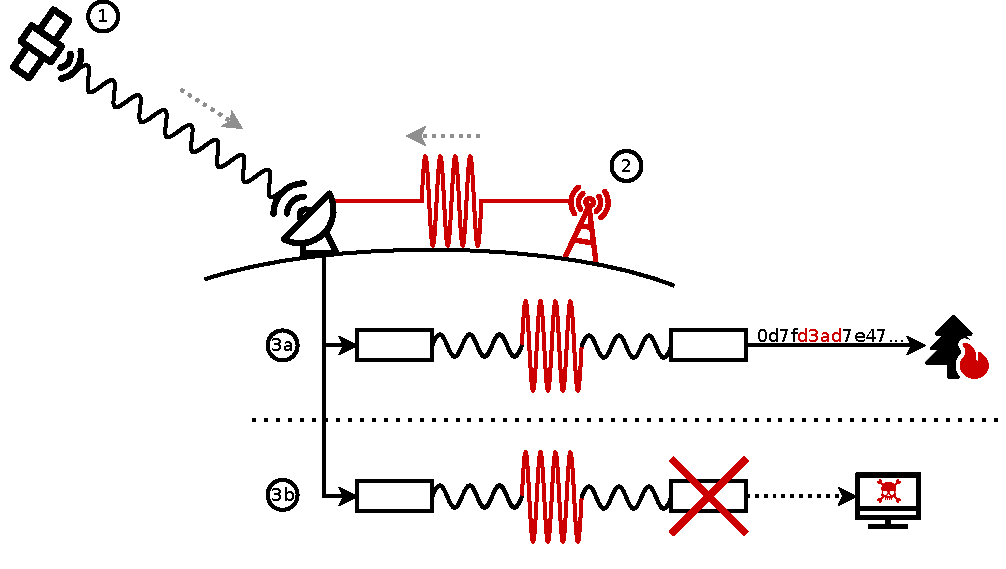
\includegraphics[width=\columnwidth]{diagrams/attack_illustration.pdf}
    \caption{An illustration of the attacks described in this paper. The attacker is indicated in red. 1)~The satellite broadcasts a signal; 2)~A ground-based attacker injects a crafted signal, overshadowing the legitimate signal and resulting in one of two scenarios; 3a)~The victim receiver decodes the attacker-controlled data, poisoning derived datasets; 3b)~The injected signal exploits vulnerabilities in the protocol decoders, resulting in denial of service or arbitrary code execution.}
    \label{fig:attack-illustration}
\end{figure}

Earth observing satellite systems are widely used in a variety of contexts, providing high-resolution images and sensor readings available within hours or less of the initial readings being taken.
Accordingly, a growing market for satellite-derived datasets has emerged which process data for specific purposes including forest fire monitoring~\cite{nasaFirms}, dust storm detection~\cite{sarikhani2021new}, and flood tracking~\cite{cloudToStreet}.
Table~\ref{tab:satellite-derived-datasets} summarizes a number of currently available satellite-derived datasets, which are derived from a mixture of self-operated, commercial, and open access satellites.

NASA's \textit{Fire Information and Resource Management System} (FIRMS) is one such use case for satellite-derived data, providing a real-time fire notification service which is used for emergency response, disaster planning, and crisis analysis, and is sent to users in more than 160 countries~\cite{firmsUsage}.
FIRMS depends on data derived from the Earth Observing System (EOS) fleet to detect precise locations of fires; an example of a surface image overlaid with detected fires is seen in Figure~\ref{fig:bushfire}.
This is possible because certain satellites in the EOS fleet contain instruments such as the \textit{Moderate Resolution Imaging Spectroradiometer} (MODIS), which provide near real time calibrated light readings across frequency bands wider than the visible spectrum.
The presence of a fire is primarily indicated by high amplitudes in the infrared bands~\cite{mod14Manual}.

Specifically, the MODIS instruments are on board \textit{Terra} and \textit{Aqua}, two EOS fleet satellites.
Thanks to their opposite polar sun-synchronous orbits, Terra and Aqua together image the entire surface of the Earth each day.
The data is downlinked to receiver stations across the world in a continuous stream known as \textit{direct broadcast}, and also as a buffered data dump to a few select locations.
As a result, MODIS data is widely available both from the central NASA archives~\cite{ladsweb} and from any of the 168 alternative receiver stations~\cite{nasaDirect}.

Even though Terra and Aqua were launched in 1999 and 2002 respectively, MODIS-derived datasets continue to see current usage across a wide variety of fields.
The satellites have a wide array of useful sensors and missions tend towards long lifespans, remaining useful for many decades.
For example, MODIS datasets continue to be used to improve fire detection algorithms, and more recently have been used to analyze weather-dispersed diseases that pose serious risks to human health~\cite{valleyFever}.

However, over the last few decades, attitudes towards securing the wireless channel in communications systems have changed significantly.
Previously, overshadowing the signal to inject data or deny service would have required a costly and highly specialized setup; since the advent of the software-defined radio, such attacks now only require access to hardware available off-the-shelf.
It is now commonly known that, using this hardware, attackers can leverage overshadowing to manipulate communications or deny service in areas such as mobile internet~\cite{yang2019hiding,erni2021adaptover}, GNSS~\cite{tippenhauer2011requirements}, and even the instruments onboard aircraft~\cite{sathayeWireless2019}.
In each of these cases a lack of robust cryptography in the system has opened it up to attack.

% TODO: insert diagram of common space comms protocols
% TODO: find out which other satellites are unencrypted, and especially those which are new and use CCSDS
% Are they generally encrypted above the CCSDS layer?

Many Earth observing satellites face similar issues, since these systems were built at a time when robust cryptography was uncommon due to less powerful onboard computers.
Therefore, while it is unsurprising that such systems are not resilient against modern adversaries, it is surprising that safety-critical infrastructure depends upon the resulting data.
These satellites include NASA's Earth Observing Fleet and NOAA's GOES fleet, which provide no cryptographic authenticity guarantees.
They also include satellites which only implement partial or now-insecure cryptography, or those whose keys have been leaked.

% TODO: summary paragraph of these
For example, the Korean satellite COMS-1 uses single DES encryption~\cite{lrit-key-dec}, which has led to customer keys being successfully extracted from satellite data.
Additionally, the GEO-KOMPSAT-2A satellite had its keys leaked on the Korea Meteorological Administration website, which to this day remain publicly available~\cite{xrit-rx}.
We should continue to expect that more encrypted satellite communications become publicly decryptable, as once-secure encryption standards and practices result in leaked encryption keys, some of which will be irrevocably baked into the firmware.

Due to the processing power constraints of the time and a desire to make the data open access, Terra and Aqua downlink their data in the clear, without employing any cryptography.
Therefore, modern off-the-shelf radio hardware enables attackers to overshadow and manipulate the raw data.
This can result in derived datasets poisoned with false information, with the processing pipeline stages themselves also potentially exploitable.

We proceed to precisely define the nature of the threat in Section~\ref{sec:threat-model}.
Using FIRMS as a case study, we describe how the attacker can poison the derived datasets and exploit the processing stages in section~\ref{sec:attack}.
This results in arbitrary manipulation of the fire detection algorithm, and denial of service and arbitrary code execution on the processing software.
We go on to validate the feasibility of the overshadowing approach in Section~\ref{sec:evaluation}, considering the case of a terrestrial attacker against a highly directional dish.

\begin{figure}
    \centering
    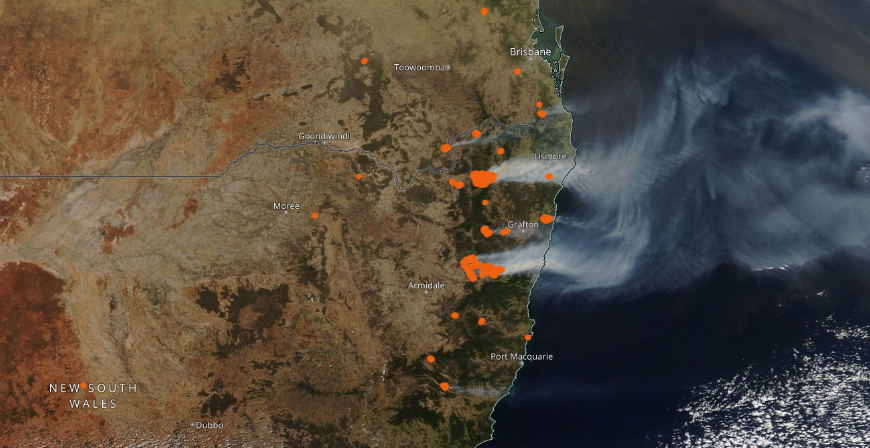
\includegraphics[width=\columnwidth]{diagrams/bushfire.png}
    \caption{The 2019 Australia bushfires as seen from Aqua's MODIS instrument, annotated with the \textit{Fires and Thermal Anomalies} dataset on NASA's worldview.\protect\footnotemark}
    \label{fig:bushfire}
\end{figure}

\footnotetext{Image taken from \url{https://worldview.earthdata.nasa.gov/?v=138.5214305912576,-37.663755528187544,165.90196079866635,-23.47436617591061\&as=2019-09-07-T00\%3A00\%3A00Z\&ae=2019-10-26-T16\%3A00\%3A00Z\&l=MODIS\_Combined\_Thermal\_Anomalies\_All,VIIRS\_SNPP\_Thermal\_Anomalies\_375m\_Day(hidden),VIIRS\_SNPP\_Thermal\_Anomalies\_375m\_Night(hidden),Reference\_Labels\_15m,Reference\_Features\_15m,Coastlines\_15m,VIIRS\_SNPP\_CorrectedReflectance\_TrueColor(hidden),MODIS\_Aqua\_CorrectedReflectance\_TrueColor,MODIS\_Terra\_CorrectedReflectance\_TrueColor(hidden)\&lg=false\&al=true\&av=3.5\&ab=on\&t=2019-09-07-T02\%3A00\%3A00Z}}


\begin{table*}
    \resizebox{\textwidth}{!}{%
    \begin{tabular}{lllll}
        \toprule
                     &       & \multicolumn{2}{c}{Satellites} & \\
        \cmidrule(lr){3-4}
        Organization & Usage & Provider & Nature & Data Access \\
        \midrule
        Planet Labs~\cite{planetProducts} & Various (intelligence, infrastructure, & Planet Labs & Self-operated & Commercial \\
                    & land use, water use) & & & \\
        Global Forest Watch~\cite{gfwMap} & Forest monitoring, carbon use, deforestation & Planet Labs & Commercial & Open access \\
        California Forest Observatory~\cite{cfoMap} & Monitoring forest fires in California & Planet Labs & Commercial & Open access \\
        ESRI~\cite{esriMap} & Land-use and land-cover maps & ESA (Sentinel-2) & Open access & Open access \\
        %Salo Sciences (TODO only bring back if I can say something about "forest restoration monitoring" project) & Conservation, climate monitoring & Planet Labs & Commercial & \\
        Meta~\cite{metaMap} & Population density maps & DigitalGlobe & Commercial & Open access \\
        Cloud to Street~\cite{cloudToStreet} & Flood tracking (disasters and insurance) & NASA (Terra/Aqua) & Open access & Commercial \\
        NCX Basemap~\cite{ncxBasemap} & Timber and carbon value monitoring in the USA & NASA & Open access & Commercial \\
        Upstream Tech HydroForecast~\cite{hydroforecast} & Water flow and weather intelligence & NASA (Terra/Aqua) & Open access & Commercial \\
        NASA FIRMS~\cite{nasaFirms} & Fire detection and management & NASA (EOS) & Self-operated & Open access \\
        \bottomrule
    \end{tabular}
    }
    \caption{Information on a number of satellite-derived datasets, including the satellite providers used to source the data.}
    \label{tab:satellite-derived-datasets}
\end{table*}


\subsection{Related Work}

Much existing work within spoofing and jamming satellite communications focuses on Global Navigation Satellite Systems (GNSS).
The authors of~\cite{wuSpoofing2020} provide a comprehensive review of known types of spoofing and jamming attacks against these satellites, resulting in incorrectly reported positions and denial of service respectively.
Spoofing attacks are carried out by a variety of methods including replay and forgery in order to fool the receiver into accepting illegitimate messages, and jamming is typically performed using high-power interference.
This work also includes a review of methods by which spoofing and jamming can be detected or mitigated.
These methods include consistency checking, measuring signal characteristics, measuring arrival times~\cite{jedermann2021orbit}, utilizing arrays of antennas, measuring angle of signal arrival, and other factors extracted through machine learning techniques~\cite{oligeri2020past}.

In contrast to GNSS systems' continuous broadcast of raw signals, the systems we are investigating are packet-based, implementing a more complex protocol stack.
We apply spoofing and jamming concepts (and their associated countermeasures) to this novel target; we demonstrate that signal spoofing is possible for satellites for which the receiving and broadcasting equipment was previously thought to make such attacks prohibitively expensive, and show that attacks can have a significant effect on processing systems downstream from the original data.
We also look beyond the payload, analyzing the data processing system itself to create novel attacks.
In Section~\ref{sec:countermeasures} we explore how an existing system might apply known countermeasures, or adapt countermeasures from related fields, to reduce the attack surface of existing satellite systems.

There is also work in satellite security beyond GNSS -- in 2020 it was demonstrated that confidential maritime satellite communications could be reveived by SDR-equipped attackers from a great distance away (covering a total area of tens of millions of square kilometers), thanks to the satellites' wide beamwidth and unencrypted payload~\cite{pavurTale2020}.
This work also explores the theoretical possibilities of TCP session hijacking by broadcasting signals over a high-speed wired connection.
Our work differs in this respect -- we focus on an attacker capable of injecting signals directly over the radio link, compromising trust in the received signal.

Finally, we consider work in physical-layer radio security beyond the scope of satellite communication.
There are a number of deployed radio systems which do not employ cryptography, including the ``ADS-B'' protocol used to locate and track aircraft.
There is a good amount of research into the security of ADS-B: \cite{strohmeierSecurity2015} provides a good review of the extent to which the system is vulnerable and explores ways to make the system more secure through verifying the transmitter location or identity, or using cryptographic methods.
Once again, we can recontextualize a number of these techniques to provide improvements to the security of other unsecured systems, which we see in Section~\ref{sec:countermeasures}.

% To go in the attack description:
\begin{comment}
The data is downlinked in almost exactly the same format for both the main data dump and the direct broadcast.
Packets from the MODIS instrument are encapsulated wthin the CCSDS Space Packet Protocol (SPP), which are packed within an unencrypted custom data link protocol known as the \textit{Channel Access Data Unit}, or CADU.
Finally, the CADUs are modulated using \textit{Quadrature Phase Shift Keying} (QPSK) and transmitted on the X-band, centered at 8160\,MHz. \textbf{TODO: is this the same for both DB and TDRSS dump?}

% TODO: is such an in-depth explanation required here?
The raw SPP packet data is known as \textit{Level 0}, and is processed through a chain of programs distributed through the IPOPP framework to generate higher-level satellite-derived datasets.
The other EOS fleet satellites are processed in much the same way.
The Level 0 data is processed into \textit{Level 1}: an easier to use heirarchical data format, optionally geolocated to a subpixel accuracy using timing information, the satellite's orbital parameters, and an accurate model of the Earth's surface.
Level 1 data is processed into a variety of \textit{Level 2} datasets, including fire detection, land surface temperature values, vegetation detection, etc.
Finally, certain Level 3 datasets are produced, which generally consist of composites of the Level 2 data for specific purposes, such as analysing post-fire burned areas.
\end{comment}

% Tasked vs untasked images - aka when you have to ask to point the satellite, vs it just gets everything
